\chapter{High-energy nuclear physics}
\section{Quantum Chromodynamics}
In the mid-20$^{\mathrm{th}}$ century, the realm of particle physics underwent a transformative phase, marked by the discovery of a seemingly endless variety of subatomic particles. This era witnessed the unveiling of numerous mesons and baryons, which left physicists with the necessity of developing a framework which could describe the behaviour of these particles and their interactions. This led to the development of the static quark model, which emerged in the 1960s as a groundbreaking conceptual framework to categorize the various observed particles. Developed independently by Murray Gell-Mann\cite{Gell-Mann:1964ewy} and George Zweig\cite{Zweig:1964jf, Fritzsch:1972jv}, this model postulated the existence of fundamental constituents called quarks, which, in order to reflect the experimental findings, had to be fermions (to describe baryons with spin 1/2 and 3/2) with fractional electric charge. The quark model beautifully explained the organization of hadrons in terms of three quarks ($u$, $d$ and $s$), leading to the development of a more structured and coherent classification of particles.

Despite the phenomenological success of the static quark model, it had two problems: it introduced particles with fractional charge, which had never been observed before, and, most importantly, it gave rise to violation of the Fermi-Dirac statistics. The $\Delta^{++}$, $\Delta^{-}$, and $\Omega^{-}$ baryons, in fact, have symmetric orbital, spin and flavour wavefunctions, which defied the Pauli exclusion principle that should have implied antisymmetric wavefunctions for these particles.

To resolve these inconsistencies, a new degree of freedom, the \emph{colour}, was introduced. Hadrons wavefunctions were assumed to be totally antisymmetric in colour quantum numbers, effectively implementing the Pauli exclusion principle.

The simplest model of colour would be to assign quarks to the fundamental representation of a global $SU(3)$ symmetry. Each quark now carries a colour index: $q_i$, where $i = 1, 2, 3$, and transforms under the fundamental ($3$) representation of $SU(3)$, while antiquarks,  $\bar{q}_i$, transform in the $\bar{3}$ representation. Introducing the totally antisymmetric tensor $\varepsilon^{ijk}$, possible compositions of quarks which give rise to colour singlets are 
\begin{equation*}
    \bar{q}^iq_i,\qquad \varepsilon^{ijk}q_iq_jq_k,\qquad \varepsilon^{ijk}\bar{q_i}\bar{q_j}\bar{q_k},
\end{equation*}
which are the quarks compositions of mesons, baryons and antibaryons, respectively. 

One of the tests supporting the existence of colour and fractional electric charge came in the form of the ratio R, of the $\mathrm{e}^+ \mathrm{e}^-$ total hadronic cross section to the cross section of a pair of muons produced from the same annihilation process. The virtual photon emitted in the annihilation can produce all electrically charged pairs of particles and antiparticles, as shown in Fig.~\ref{fig:ee_to_ff_diagram}.

\begin{figure}[h]
    \centering
        \feynmandiagram [horizontal=a to b] {
          i1 [particle=\(e^{-}\)] -- [fermion] a -- [fermion] i2 [particle=\(e^{+}\)],
          a -- [photon, edge label=\(\gamma^*\)] b,
          f1 [particle=\(\bar{f}\)] -- [fermion] b -- [fermion] f2 [particle=\(f\)],
        };
\caption{$\mathrm{e}^+ \mathrm{e}^-$ annihilation to a pair of fermions}
    \label{fig:ee_to_ff_diagram}
\end{figure}


The ratio R is given by:
\begin{equation*}
    R = \frac{\sigma(e^+e^- \rightarrow hadrons)}{\sigma(e^+e^- \rightarrow \mu^+\mu^-)} = N_c \sum_f Q_f^2\ ,
\end{equation*}
where $N_c$ represents the number of existing colours and and $Q_f$ is the electric charge of the quark flavour $f$. Notably, this ratio is dependent on the energy of the center-of-mass system and encompasses all possible quark flavors that can be produced by the virtual photon at that specific energy level. The experimental data for $R$ (shown in Fig.~\ref{fig:R_vs_s}) exhibited a remarkable agreement with the predictions of the three-color model, thereby providing compelling evidence for the existence of color and fractional electric charge of quarks.

The final step that propelled the development of QCD as a comprehensive theory of the strong force was the insight into the mechanism that ensured all hadron wavefunctions to be color singlets. This emerged from the discovery of asymptotic freedom, a phenomenon observed in deep-inelastic scattering experiments. Non-Abelian gauge theories, often referred to as Yang-Mills theories, were identified as having this unique characteristic. This realization led to the formulation of QCD by elevating the global color $SU(3)$ symmetry to a local one, allowing the 8 quanta of the $SU(3)$ gauge field, called \emph{gluons}, to mediate the strong force, successfully describing the confinement and behavior of quarks and gluons within hadrons.

\begin{figure}[p]
    \centering
    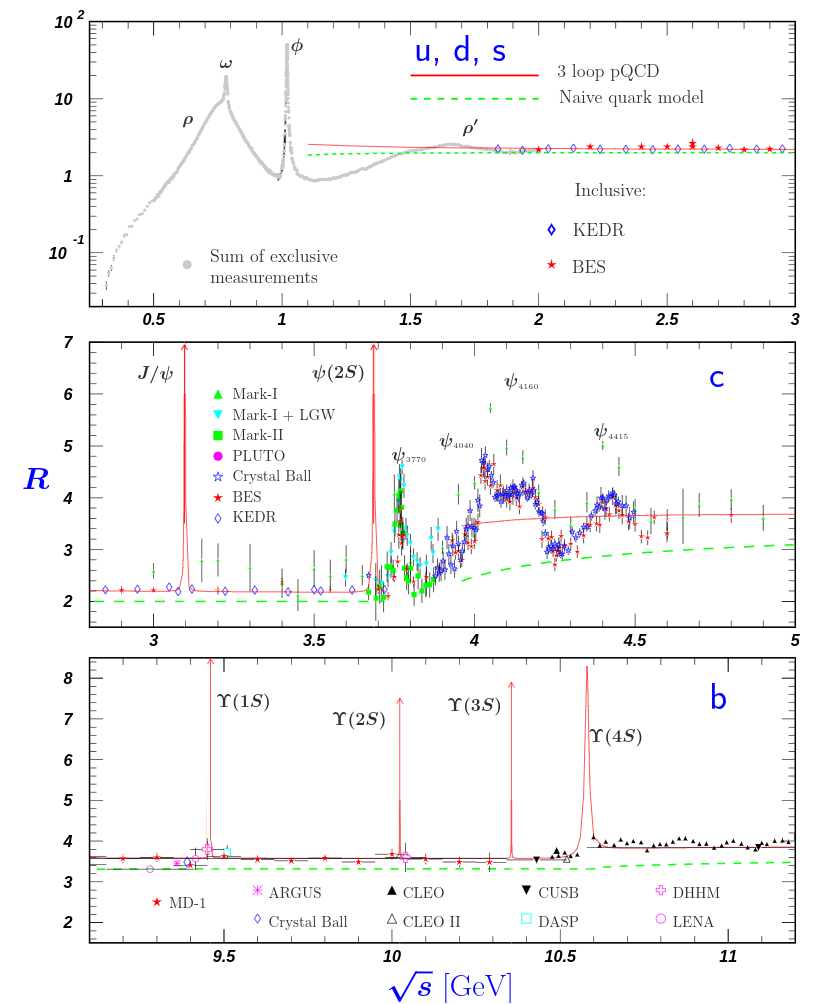
\includegraphics[width=\linewidth]{Figures/Chapter 1/rpp2022-R_udscb.pdf}
    \caption{$R$ as a function of $\sqrt{s}$ in the light-flavor, charm, and beauty threshold regions taken from \cite{pdg}. The green curve is a naive quark-parton model prediction, while the red one is 3-loop pQCD prediction. Breit-Wigner parameterizations of $J/\psi$, $\psi$(2S), and $\Upsilon$(nS), n = 1,2,3,4 are also shown}
    \label{fig:R_vs_s}
\end{figure}

The QCD Lagrangian density can be written as:
\begin{equation}\label{eq:Lqcd}
    \mathcal{L}_{QCD}=-\frac{1}{4} F^a_{\mu\nu}F_a^{\mu\nu} + \sum_f \bar{q}_f^i (i\gamma^\mu(\mathcal{D}_\mu)_{ij}-m_f\delta_{ij})q_f^j\ ,
\end{equation}
where $F^a_{\mu\nu}$ is the field strength tensor defined in terms of the gluon field $A^a_\mu$ and the $SU(3)$ structure constant $f^{abc}$:
\begin{equation} \label{eq:F}
    F^a_{\mu\nu} = \partial_\mu A^a_\nu - \partial_\nu A^a_\mu + g_s f^{abc}A^b_\mu A^c_\nu 
\end{equation}
and $(\mathcal{D}_\mu)_{ij}$ is the covariant derivative:
\begin{equation*}
    (\mathcal{D}_\mu)_{ij} = \partial_\mu \delta_{ij} - ig_s(t^a)_{ij}A_\mu^a\ ,
\end{equation*}
with $t^a$ being one of the generators of the $SU(3)$ representation.

The last term in Eq.~\ref{eq:F} is peculiar of non-Abelian theories, and gives rise to triplet and quartic gluon self-interactions illustrated in Fig.~\ref{fig:Feynman-gluons}. $g_s$ is the coupling constant, which determines the strenght of the interaction between the coloured particles.

\begin{figure}[htb]
    \centering
    \begin{tikzpicture}
      \begin{feynman}
        \vertex (a) {a};
        \vertex [right=of a] (b);
        \vertex[above right= of b] (c) {b};
        \vertex[below right= of b] (d) {c};
        \diagram* {
          (a) -- [gluon] (b),
          (b) -- [gluon] (c),
          (b) -- [gluon] (d),
        };
      \end{feynman}
    \end{tikzpicture} \qquad
    \begin{tikzpicture}
      \begin{feynman}
        \vertex (a);
        \vertex[above left=of a] (b) {a};
        \vertex[above right= of a] (c) {b};
        \vertex[below right= of a] (d) {c};
        \vertex[below left= of a] (e) {d};
        \diagram* {
          (a) -- [gluon] (b),
          (a) -- [gluon] (c),
          (a) -- [gluon] (d),
          (a) -- [gluon] (e),
        };
      \end{feynman}
    \end{tikzpicture}
    \caption{Feynman diagrams for gluons self-interactions}
    \label{fig:Feynman-gluons}
\end{figure}

The second term of Eq.~\ref{eq:Lqcd} describes the interactions between quarks and gluons, sketched in Fig.~\ref{fig:Feynman_q_g}, and contains the mass term for the fermions. It is noteworthy to observe that the interaction between quarks and gluons is diagonal in flavor, meaning that the strong interaction conserves the flavor of quarks. In contrast, colour mixing is allowed within the framework of QCD.

\begin{figure}[htb]
    \centering
    \begin{tikzpicture}
      \begin{feynman}
        \vertex (a);
        \vertex [below=0.1em of a] {$t^a_{ij}$};
        \vertex[left=of a] (b) {$q_i$};
        \vertex[right= of a] (c) {$q_j$};
        \vertex[above right= of a] (d) {a};
        \diagram* {
          (b) -- [fermion] (a),
          (a) -- [fermion] (c),
          (a) -- [gluon] (d),
        };
      \end{feynman}
    \end{tikzpicture}
    \caption{Feynman diagram for quark-gluon interaction}
    \label{fig:Feynman_q_g}
\end{figure}

\subsection{Running coupling constant}
If one considers a dimensionless physical observable, denoted in the following as $R$, which solely depends on a single energy scale, $Q$, one might naturally expect that $R$ would maintain a constant value, independent of the specific energy scale chosen. However, this does not hold true when loop diagrams are studied: the necessity of renormalisation introduces a new energy scale denoted as $\mu$. This scale, known as the renormalisation scale, is the point at which the subtraction of the ultraviolet divergences is carried out. Critically, $\mu$ is an arbitrary parameter and, as such, is non-physical. Consequently, $R$ becomes dependent on the ratio $Q^2/\mu^2$ and the renormalised coupling $\alpha_s = g_s^2/4\pi$: $R = R\left(\frac{Q^2}{\mu^2},\als\right)$. The $\mu$ independence of $R$ (which is an essential requirement given $\mu$'s arbitrariness) can be expressed as:
\begin{equation}\label{eq:RGE}
    \mu^2 \frac{\de R\left(\frac{Q^2}{\mu^2},\alpha_s\right)}{\de \mu^2} = \mu^2 \left[\frac{\partial}{\partial\mu^2}+\frac{\partial \alpha_s}{\partial\mu^2}\frac{\partial}{\partial\alpha_s}\right]R\left(\frac{Q^2}{\mu^2},\alpha_s\right) = 0\ , 
\end{equation}
a fundamental equation known as the renormalisation group equation. This equation holds true in the case of a prediction which considers all perturbative orders. If one limits the expansion at a fixed order $\alpha_s^N$, then a dependence of $R$ from $\mu$ is observed at the $\als^{N+1}$ order.\\ Solving Eq.~\ref{eq:RGE} requires the introduction of the concept of the running coupling $\alpha_s(Q^2)$, which evolves as a function of $Q$. By introducing
\begin{equation*}
    t\equiv \mathrm{log}(Q^2/\mu^2), \qquad \beta(\als)\equiv \mu^2 \frac{\de\als}{\mathrm{\mu^2}}\quad ,
\end{equation*}
Eq.~\ref{eq:RGE} can be written as
\begin{equation*}
    \left(-\frac{\partial}{\partial t} + \beta(\als)\frac{\partial}{\partial \als}\right) R(e^t,\als) = 0
\end{equation*}
This first order partial differential equation can be solved by defining a new function: the running coupling $\als(Q^2)$
\begin{equation}\label{eq:t_integral}
    t = \mathrm{log}(Q^2/\mu^2) \equiv \int_{\als}^{\als(Q^2)} \frac{\de x}{\beta(x)} , \quad \mathrm{with}~\als=\als(\mu^2)\quad .
\end{equation}
By differentiating Eq.~\ref{eq:t_integral} with respect to $t$ and \als, one gets:
\begin{equation}\label{eq:beta_def}
    \beta(\als(Q^2)) = \frac{\partial\als(Q^2)}{\partial t}, \quad \frac{\de\als(Q^2)}{\de\als} = \frac{\beta(\als (Q^2))}{\beta(\als))}\quad .
\end{equation}
It results from this last set of equations that $R(1,\als(Q^2))$ satisfies Eq.~\ref{eq:RGE}; hence, the running coupling constant has absorbed the $\mu$ scale dependence of $R$. As a consequence, the knowledge of $R(1,\als)$, which can be evaluated in fixed-order perturbation theory, allows to know the dependence of $R$ from $Q^2$, which is the physical scale at which the coupling is gauged, by simply substituting $\als \rightarrow \als(Q^2)$. 

\subsubsection{The \ensuremath{\beta} function}
The running of the coupling constant is determined by the $\beta(\als)$ function, which is evaluated from loop corrections to the bare vertices of the theory. As of the time of the writing of this Thesis, the $\beta$ function has been evaluated up to 5 loops\cite{Herzog:2017ohr}. In Fig.~\ref{fig:beta_loops}, the 1-loop Feynman diagrams contributing to the $\beta$ function evaluation are reported.

\begin{figure}[htb]
    \centering
    \begin{tikzpicture}
      \begin{feynman}
        \vertex (a);
        \vertex [right=1cm of a] (b);
        \vertex[right=1cm of b] (c);
        \vertex[right=1cm of c] (d);
        \diagram* {
            (a) -- [gluon] (b)
            -- [fermion, half left, looseness=1.5] (c)
            -- [fermion, half left, looseness=1.5] (b),
            (c) -- [gluon] (d),
        };
      \end{feynman}
    \end{tikzpicture}\quad
    \begin{tikzpicture}
      \begin{feynman}
        \vertex (a);
        \vertex [right=1cm of a] (b);
        \vertex[right=1cm of b] (c);
        \vertex[right=1cm of c] (d);
        \diagram* {
            (a) -- [gluon] (b)
            -- [gluon, half left, looseness=1.5] (c)
            -- [gluon, half left, looseness=1.5] (b),
            (c) -- [gluon] (d),
        };
      \end{feynman}
    \end{tikzpicture}\quad
    \begin{tikzpicture}
      \begin{feynman}
        \vertex (a);
        \vertex [right=of a] (b);
        \vertex[above=1cm of b] (c);
        \vertex[right=of b] (d);
        \diagram* {
            (a) -- [gluon] (b)
            -- [gluon, half left, looseness=1.5] (c)
            -- [gluon, half left, looseness=1.5] (b),
            (b) -- [gluon] (d),
        };
      \end{feynman}
    \end{tikzpicture}\quad

    \vspace{0.6cm}
    \begin{tikzpicture}
      \begin{feynman}
        \vertex (a);
        \vertex [right=1cm of a] (b);
        \vertex[right=1cm of b] (c);
        \vertex[right=1cm of c] (d);
        \diagram* {
            (a) -- [gluon] (b)
            -- [ghost, half left, looseness=1.5] (c)
            -- [ghost, half left, looseness=1.5] (b),
            (c) -- [gluon] (d),
        };
      \end{feynman}
    \end{tikzpicture}\quad
    \begin{tikzpicture}
      \begin{feynman}
        \vertex (a);
        \vertex [right=1cm of a] (b);
        \vertex[right=1cm of b] (c);
        \vertex[right=1cm of c] (d);
        \vertex[below=0.31cm of c] (f) {$ $};
        \diagram* {
            (a) -- [fermion] (b) -- [fermion] (c) -- [fermion] (d),
            (b) -- [gluon, half left, looseness=1.5] (c)
            
        };
      \end{feynman}
    \end{tikzpicture}\quad
    
    \vspace{0.5cm}
    \begin{tikzpicture}
      \begin{feynman}
        \vertex (a);
        \vertex [right=1cm of a] (b);
        \vertex[above right=1cm of b] (c);
        \vertex[right=1cm of c] (d);
        \vertex[below right=1cm of b] (e);
        \vertex[right=1cm of e] (f);
        \diagram* {
            (a) -- [gluon] (b) -- [fermion] (c) -- [fermion] (d),
            (b) -- [fermion] (e) -- [fermion] (f),
            (c) -- [gluon] (e)
        };
      \end{feynman}
    \end{tikzpicture}\quad
    \begin{tikzpicture}
      \begin{feynman}
        \vertex (a);
        \vertex [right=1cm of a] (b);
        \vertex[above right=1cm of b] (c);
        \vertex[right=1cm of c] (d);
        \vertex[below right=1cm of b] (e);
        \vertex[right=1cm of e] (f);
        \diagram* {
            (a) -- [gluon] (b) -- [gluon] (c),
            (b) -- [gluon] (e),
            (f) -- [fermion] (e) -- [fermion] (c) -- [fermion] (d)
        };
      \end{feynman}
    \end{tikzpicture}\quad
    \caption{1-loop Feynman diagrams contributing to the $\beta$ function evaluation}
    \label{fig:beta_loops}
\end{figure}

By limiting the calculations at the first order in the perturbative expansion, one gets:
\begin{equation}\label{eq:beta0}
    \beta(\als) = -\als^2 \frac{11 \mathrm{N_c} - 2 \mathrm{N_f}}{12\pi} + \mathcal{O}(\als^3) \equiv -\als^2 \beta_0 + \mathcal{O}(\als^3)\quad ,
\end{equation}
where $\mathrm{N_c}$ is the number of colours (3), while $\mathrm{N_f}$ is the number of quark flavours which can be considered massless at the physical scale $Q^2$ at which the coupling is being measured.
From Eqs.~\ref{eq:beta0} and \ref{eq:beta_def}, one can extract the $Q^2$ dependency of the running coupling constant:
\begin{equation*}
    \alpha_s(Q^2) = \frac{\alpha_s(\mu^2)}{1+\alpha_s(\mu^2)\beta_0 \mathrm{log}(Q^2/\mu^2)}\ ,
\end{equation*}
Notably, since $\beta_0$ is positive also when considering 6 quark flavours, the strong coupling constant exhibits a monotonic decreasing trend as a function of $Q^2$



AGGIUNGERE $\Lambda_{QCD}$ e parlare della libertà asintotica e del confinamento!!!